\documentclass[11pt]{article}
\usepackage[utf8]{inputenc} % Para caracteres en espa�ol
\usepackage{amsmath,amsthm,amsfonts,amssymb,amscd}
\usepackage{multirow,booktabs}
\usepackage[table]{xcolor}
\usepackage{fullpage}
\usepackage{lastpage}
\usepackage{enumitem}
\usepackage{multicol}
\usepackage{fancyhdr}
\usepackage{mathrsfs}
\usepackage{wrapfig}
\usepackage{setspace}
\usepackage{esvect}
\usepackage{calc}
\usepackage{multicol}
\usepackage{cancel}
\usepackage{graphicx}
\graphicspath{ {pictures/} }
\usepackage[retainorgcmds]{IEEEtrantools}
\usepackage[margin=3cm]{geometry}
\usepackage{amsmath}
\newlength{\tabcont}
\setlength{\parindent}{0.0in}
\setlength{\parskip}{0.05in}
\usepackage{empheq}
\usepackage{framed}
\usepackage[most]{tcolorbox}
\usepackage{xcolor}
\colorlet{shadecolor}{orange!15}
\parindent 0in
\parskip 12pt
\geometry{margin=1in, headsep=0.25in}
\theoremstyle{definition}
\newtheorem{defn}{Definition}
\newtheorem{reg}{Rule}
\newtheorem{exer}{Exercise}
\newtheorem{note}{Note}
\newcommand{\volume}{{\ooalign{\hfil$V$\hfil\cr\kern0.08em--\hfil\cr}}}
\newcommand{\parr}{\mathbin{\|}} % Parralel Symbol
\begin{document}
\setcounter{section}{0}
\setcounter{page}{0}
\setcounter{equation}{0}
%\definecolor{babyblue}{rgb}{0.54, 0.81, 0.94}
\definecolor{babyblueeyes}{rgb}{0.63, 0.79, 0.95}
\definecolor{babyblue}{rgb}{0.69, 0.88, 0.9}

 \pagestyle{fancy}
\fancyhf{}
\rhead{Section 3: Electrical Conductivity}
\rfoot{Page \thepage}
\thispagestyle{empty}


\begin{center}
{\LARGE \bf Section 3: Electrical Conductivity}\\
{\large AE435}\\
Spring 2018
\end{center}
In this unit, we will explore electrical conductivity within an ionized gas.
That is, a gas that consists of charged particles that can freely move
under the influence of their own inertia, and whose motion will be
influenced by body forces (Electric and Magnetic forces, ignoring
gravity) and momentum-transfer collisions (with other particles,
with boundaries).

In the presence of both electric and magnetic fields, the
constitutive equation for conductivity is:
\newline \begin{equation}
\begin{aligned}
\vv{j} = \sigma (\vv{E}+\vv{v} \times \vv{B})
\end{aligned}
\end{equation}\newline
While the definition of current density is:
\newline \begin{equation}
\begin{aligned}
\vv{j} = \sum_i n_i \, q_i \, \vv{v_i}
\end{aligned}
\end{equation}\newline
Where $i$ denotes one of the species in the plasma, and $\vv{v_i}$ is the
\textbf{drift velocity}, or mean velocity for species $i$ .

Conductivity is really determined by the equation of motion for
charge carriers, including:
\begin{itemize}
\item Inertia term
\item Body forces
\item Momentum-transfer collisions between species
\end{itemize}
We must understand how charged particles (plasma particles, ions,
electrons) move (their equation of motion) in the presence of
electric and magnetic fields, and in the presence of other particles
(collisions). We start by ignoring collisions (just analyze motion
in E and B fields), then add collisions.
\newpage
\begin{center}
\vspace{5mm}
\end{center}
\section{Charged Particle Motions}
\newline
In this section, we will look at single-particle motion. Motion of a
single particle in electric and magnetic fields.
\begin{center}
\vspace{25mm}
\end{center}
\tableofcontents
\newpage
\subsection{Uniform, Steady B-Field, No E-Field}
Start by ignoring collisions (reasonable for low density and low
temperature).

Let $\vv{B} = B \, \hat{z}$

Then Lorentz force, $\vv{F} = q \,(\vv{E} + \vv{v} \times \vv{B})$, with $\vv{E} = 0$ is:
\newline \begin{equation}
\begin{aligned}
\vv{F} = q \, \vv{v} \times \vv{B} = m \, \frac{\mathrm{d}\vv{v}}{\mathrm{d}t}
\end{aligned}
\end{equation}\newline
Looking at the $\vv{v} \times \vv{B}$ term,
\newline \begin{equation}
\begin{aligned}
\vv{v} \times \vv{B} &= (\vv{v}_y \vv{B}_z - \vv{v}_z \vv{B}_y) \hat{x} - (\vv{v}_x \vv{B}_z - \vv{v}_z \vv{B}_x) \hat{y} + (\vv{v}_x \vv{B}_y - \vv{v}_y \vv{B}_x) \hat{z} \\ \\
&= \vv{v}_y B \hat{x} - \vv{v}_x B \hat{y}
\end{aligned}
\end{equation}\newline
As a result, Equation 3 becomes
\newline \begin{equation}
\begin{aligned}
\text{x-comp: }& \quad  m \, \frac{\mathrm{d}\vv{v}_x}{\mathrm{d}t} = q \, B \, v_y = m \dot{v}_x & \\ \\ 
\text{y-comp: }& \quad  m \, \frac{\mathrm{d}\vv{v}_y}{\mathrm{d}t} = - q \, B \, v_x = m \dot{v}_y & \\ \\
\text{z-comp: }& \quad  m \, \frac{\mathrm{d}\vv{v}_z}{\mathrm{d}t} = 0 = m \dot{v}_z & \\ \\
\end{aligned}
\end{equation}\newline
So, there is NO force on the particle acting in the z-direction
(along B, of course not, B can't do work on particle). Any motion
Along B remains same.

What about motion perpendicular to B?

How about x and y motion?

Take derivative of (3.5a) and (3.5b):
\newline \begin{equation}
\begin{aligned}
m \, \ddot{v}_x = q \, B \, \dot{v}_y = - \frac{(q \, B)^2}{m} v_x \\ \\
m \, \ddot{v}_y = - q \, B \, \dot{v}_x = - \frac{(q \, B)^2}{m} v_y
\end{aligned}
\end{equation}\newpage
So
\newline \begin{equation}
\begin{aligned}
\ddot{v}_x = - (\frac{q \, B}{m})^2 v_x \\ \\
\ddot{v}_y = - (\frac{q \, B}{m})^2 v_y
\end{aligned}
\end{equation}\newline
Equations 7 takes the form of a Simple Harmonic Oscillator ($m\ddot{x} + k x = 0$) with Frequency
\newline 
\begin{shaded}
\textbf{Cyclotron/Gyro Frequency}
\begin{equation}
\begin{aligned}
\omega_B = \frac{|q| B}{m} \qquad \qquad B[T] \quad m [kg] \quad q [c]\\

\end{aligned}
\end{equation}
\end{shaded}\newline
The solution of Equation 7 is 
\newline \begin{equation*}
\begin{aligned}
v_x = C \, \cos(\omega_B t - \alpha)
\end{aligned}
\end{equation*}\newline
Where
\newline \begin{equation*}
\begin{aligned}
C &= \text{Constant} \\
\alpha &= \text{Phase Angle, choose $\alpga = 0$} \\
\end{aligned}
\end{equation*}\newline

We will introduce $v_{\perp} = \sqrt{v_x^2 + v_y^2}$ which is the amplitude of the velocity perpendicular to $\vv{B}$.

Choose at $t=0$ and $v_y = 0$ such that...
\begin{subequations}
\newline \begin{equation}
\begin{aligned}
v_x = v_{\perp} \cos(\omega_B t) = \dot{x}
\end{aligned}
\end{equation}\newline
from Equation 4a in Section 2
\newline \begin{equation}
\begin{aligned}
v_y = \mp \, \frac{1}{\omega_B}  \, \dot{v_x} = \mp  \, \frac{1}{\omega_B} \omega_B  \, v_{\perp}  \, \sin(\omega_B t) = \mp \,  v_{\perp}  \, \sin(\omega_B t) = \dot{y}
\end{aligned}
\end{equation}\newline
\end{subequations}
Where the $\pm$ or $\mp$ is the signage for an ion (top) or electron (bottom). To clarify, here, (-) is for an ion and (+) is for an electron.

Moving on, we integrate Equation 9 to get
\newline \begin{equation}
\begin{aligned}
x-x_o = \frac{v_{\perp}}{\omega_B}\sin(\omega_B t) \qquad \text{and} \qquad
y-y_o = \pm \frac{v_{\perp}}{\omega_B}\sin(\omega_B t)
\end{aligned}
\end{equation}\newline
Recall our earlier notation such that, for this case, (+) is for the ion and (-) for the electron. 
\newpage
From this, we can define 
\begin{shaded}
\textbf{Larmor/Gyro Radius}
\newline \begin{equation}
\begin{aligned}
r_L = \frac{v_{\perp}}{\omega_B} = \frac{m \, v_{\perp}}{q \, B}
\end{aligned}
\end{equation}\newline
\end{shaded}
\begin{framed}
\textbf{Plotting this motion:}
\begin{center}
\vspace{40mm}
\textbf{Figure 1}
\end{center}
We see that the particle moves in circular motion with radius $r_L$ at a frequency of $\omega_B$.
\begin{center}
 \begin{tabular}{||c | c c | c c ||} 
 \hline
 Time & Location &  (Equation 10) & Velocity & (Equation 9)\\[1ex] 
 \hline\hline
 $t=0$ & $x=0$ & $y=r_L$ & $V_x = V_{\perp}$ & $V_y = 0$\\[1.5ex] 
 $t=\frac{\pi}{2 \, \omega_B}$ & $x=r_L$ & $y=0$ & $V_x = 0$ & $V_y = -V_{\perp}$\\[1.5ex] 
 $t=\frac{\pi}{\omega_B}$& $x=0$ & $y= - r_L$ & $V_x = - V_{\perp}$ & $V_y = 0$\\[1.5ex] 
 $t=\frac{3 \, \pi}{2 \, \omega_B}$ & $x= - r_L$ & $y=0$ & $V_x = 0$ & $V_y = V_{\perp}$\\[1.5ex] 
 \hline
\end{tabular}
\end{center}
\end{framed}
To summarize: charged particles execute cyclotron motion (gyro-motion) in
magnetic fields. Frequency of this motion is $\omega_B$, the cyclotron
frequency. Radius of this circular motion is $r_L$, the Larmor
radius.

Note that ions and electrons rotate in different directions. They
move so that the Bfield due to particle motion cancels/opposes the
applied magnetic field (right hand rule).

Plasma particles tend to reduce the applied Bfield, and thus are diamagnetic.

Also remember there is a $V_z$ along B. In other words, $V_{||}$ remains constant or is unchanged.
\newpage
\subsection{Uniform, Steady B-Field and E-Field}
Now add a constant Electric field. In this case the particle motion
is composed of two parts:
\begin{enumerate}
\item Gyro-motion (Section 3, 1.1)
\item Guiding center drift
\end{enumerate}
We can choose our axes so that $\vv{B} = B \, \hat{z}$ and $\vv{E}$ lies in the
x-z plane,
\begin{center}
\vspace{40mm}
\textbf{Figure 2}
\end{center}
The lorentz force equation is our equation of motion, $\vv{F} = q \, (\vv{E} + \vv{v} \times \vv{B}) = m \frac{dv}{dt}$.

The z-component or the component along/parallel to the B-field direction is:
\newline
\newline \begin{equation}
\begin{aligned}
\frac{\mathrm{d}v_z}{\mathrm{d}t} = \frac{q}{m} E_z \\ \\
v_z = \frac{q}{m} \, E_z \, t + v_{z,0}
\end{aligned}
\end{equation}\newline
\newline
\textbf{Acceleration of the particle is along $\bf{\vv{B}}$}. $v_z = v_{||}$ changes with
time meaning it is no longer constant as before. This is due to the E-field component along $\vv{B}$ which accelerates the particle along $\vv{B}$.

The x and y components (perpendicular to B-field direction) for
\newline
\newline \begin{equation}
\begin{aligned}
\dot{v}_x &= \frac{q}{m}\,E_x \pm \omega_B \, v_y &\qquad \text{(Now has $E_x$)} \\ \\
\dot{v}_y &= 0 \pm \omega_B \, v_x &\qquad \text{(Same as Equation 5)} \\
\end{aligned}
\end{equation}\newline
\newpage
Differentiating with constant $\vv{E}$
\newline
\newline \begin{equation}
\begin{aligned}
\ddot{v}_x &= -\omega_B^2 \, v_x &\qquad \text{(Same as Equation 7)} \\ \\
\ddot{v}_y &= -\omega_B^2 \, \bigg(v_y + \frac{E_x}{B} \bigg) &\qquad \text{(Now has $E_x$)} \\
\end{aligned}
\end{equation}\newline
\newline
The solution of these equations is:
\newline
\newline \begin{equation}
\begin{aligned}
v_x = v_{\perp} \cos (\omega_B t) \\ \\
v_y = \mp v_{\perp} \sin (\omega_B t) - \frac{E_x}{B}
\end{aligned}
\end{equation}\newline
\begin{itemize}
\item Note that compared with Equation 9 from before, there is now a drift
in the -y direction (for $E_x > 0$).
\newline \begin{equation*}
\begin{aligned}
\text{Drift} = - \frac{E_x}{B}
\end{aligned}
\end{equation*}\newline
\item Even though E was only in x and z directions, it causes drift in
y direction.
\item This is called guiding center drift since the point about which
the particle gyrates is moving.
\end{itemize}
\begin{center}
\vspace{20mm}
\large{\textbf{We will now begin looking at sketches of charged particle motion.}}
\end{center}
\newpage
\textbf{Case 1:} Gyromotion that drifts in $\bf{E\times B}$ (-y) direction. Gyromotion that stays in
the x-y plane.
\newline \begin{equation*}
\begin{aligned}
\vv{B} = B \hat{z} \qquad \vv{E} = E_x \hat{x} \qquad v_{||} = v_z = 0
\end{aligned}
\end{equation*}\newline
\begin{center}
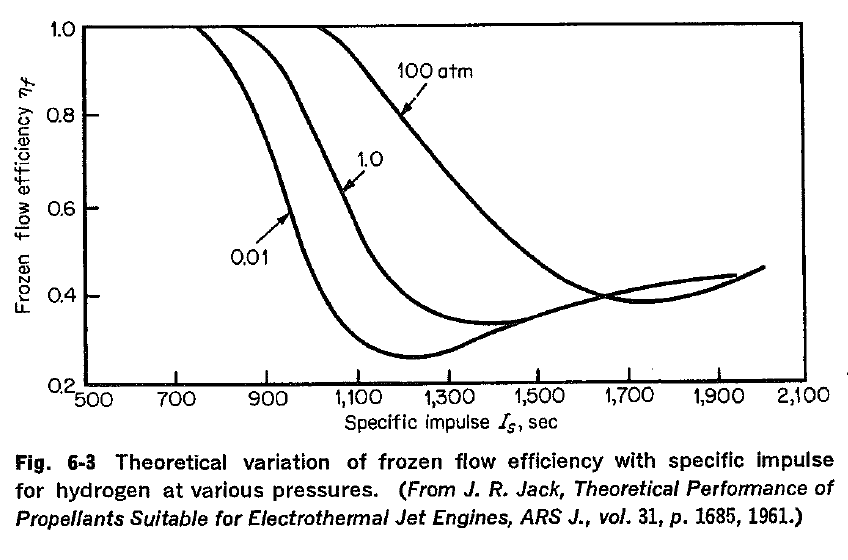
\includegraphics[scale=1]{1.png}
\end{center}
In this case, a charge is starting from rest in uniform perpendicular $\vv{E}$ and $\vv{B}$ fields. 
%What this figure is showing is that the motion in two different reference frames. Left side we are moving parralel with the drift velocity, right side is the laboratory frame, we are note moving with the guiding center. B is the y direction, and E is out of the page and so the particle is going to drift. It is doing this cyclotron motion but now the whole thing starts to move. Cyclatron motion superimposed on a drift.
Here the total force is normal to v and to B 
\begin{equation*}
\begin{aligned}
\vv{F} = q \, (\vv{E} + \vv{v} \times \vv{B}) = m \frac{dv}{dt}
\end{aligned}
\end{equation*}
and the initial velocity, $v_o$, is simply the negative of the drift velocity, $v_{\text{drift}}$.
\begin{equation*}
\begin{aligned}
v_o^1 = v_o - v_{\text{drift}} = -v_{\text{drift}} = - \frac{\vv{E} \times \vv{B}}{B^2}
\end{aligned}
\end{equation*}
The motion in a coordinate system moving with the drift velocity relative to the laboratory frame is a circle of radius:
\begin{equation*}
\begin{aligned}
r^1 = \frac{m \, v_o^1}{q \, B} = \frac{m \, v_{\text{drift}}}{q \, B} = \frac{m \, E}{q \, B^2}
\end{aligned}
\end{equation*}
which is transcribed with constant tangential speed, $v_{\text{drift}} = \frac{E}{B}$, in the plane normal to $\vv{B}$. In the laboratory frame, this motion transforms into a cycloid in the same plane, advancing in the $\vv{E} \times \vv{B}$ direction with drift speed $\frac{E}{B}$ as seen in the figure above. Note that this drift is normal to $\vv{E}$ and independent of the charge sign.
\newpage
\textbf{Case 2:} Gyromotion that drifts in the $\bf{E\times B}$ (-y) direction, with an initial
parallel velocity component. Helix with constant pitch, pushed over on its side.
\newline \begin{equation*}
\begin{aligned}
\vv{B} = B \hat{z} \qquad \vv{E} = E_x \hat{x} \qquad v_{||} = v_z \neq 0
\end{aligned}
\end{equation*}\newline
\begin{center}
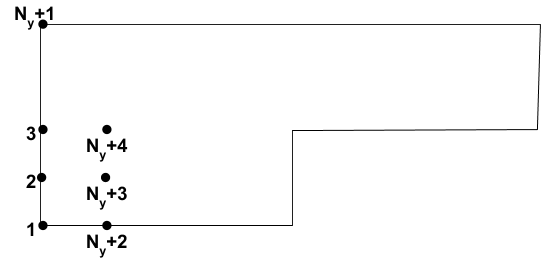
\includegraphics[scale=0.7]{2.png}
\end{center}
In this case, we now have a velocity in the z-direction. As a result it not only has a gyromotion but is also moving up at the same time. On top of that, it also is moving to the right because of our drift velocity. Note however that the velocity parallel to the z-component is constant!
\newpage
\textbf{Case 3:} Gyromotion that drifts in $\bf{E\times B}$ (-y) direction, WITH an initial
perpendicular velocity.
%Now more complicated, B in z direction, E in x direction, no velocity in z irection but has initial velocity in the x,y plane. The intitial motion that is opposite to the drift direction. 
\newline \begin{equation*}
\begin{aligned}
\vv{B} = B \hat{z} \qquad \vv{E} = E_x \hat{x} \qquad v_{||} = v_z = 0 \qquad v_{\perp,0} \neq 0
\end{aligned}
\end{equation*}\newline
\textbf{Prolate} - initial velocity opposes $E\times B$ drift

\textbf{Curtate} - initial velocity same direction as $E\times B$ drift
\begin{center}
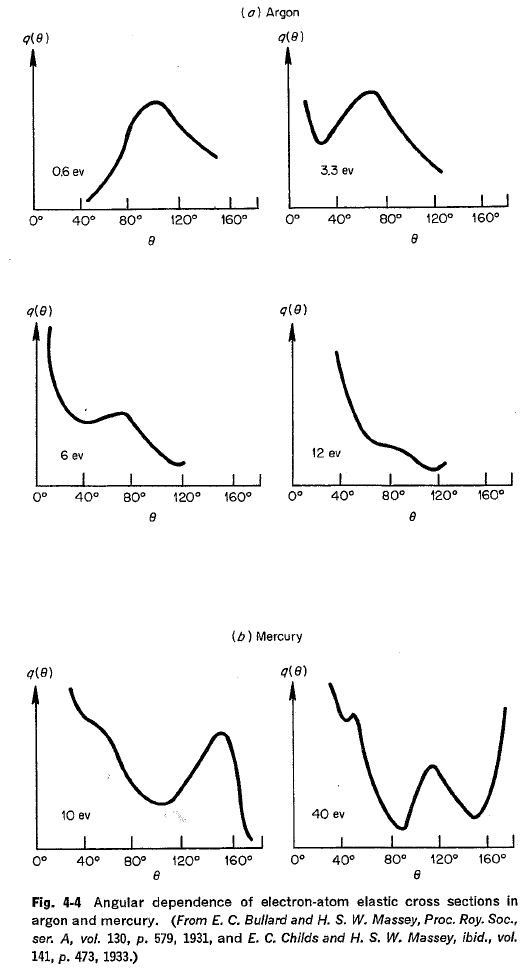
\includegraphics[scale=0.7]{3.png}
\end{center}
If $\vv{v}_o \neq 0$ but has some component parallel to $\vv{B}$, the motion in the transformed system will be a helix instead of a circle, and in the laboratory frame, an inclined helix whose axis lies in the $\vv{B}$, $\vv{E} \times \vv{B}$ plane. If $\vv{v}_o$ also has a component normal to $\vv{B}$, this will contribute to the $\vv{v}^1 \times \vv{B}$ force, and hence, change the radius of gyration and angular velocity, without affecting the drift velocity. The orbit then becomes a prolate cycloid (i.e. has loops) or a curtate cycloid depending on $\vv{v}^1_{0,\perp} \lessgtr \frac{E}{B}$. The cycloid always progresses along the positive $\vv{E} \times \vv{B}$ axis, but its position relative to that axis depends on the direction of $\vv{v}^1_{0,\perp}$.

\textbf{Note:} the very special case of $\vv{v}^1_o = 0$, that is, $\vv{v}_o = v_{\text{drift}}} = (\vv{E} \times \vv{B})/B^2$. A particle injected with this velocity moves in a straight line, undisturbed by the fields.
\newpage
\textbf{Case 4:} Gyromotion with drift, with acceleration along B.
\newline \begin{equation*}
% Now adding all the cases together. Now we have B in z direction, E in x and z direction. There could be an initial parallel velocity but it doesnt really matter, trajectory would look the same. Becasue we have a b feld the. Particle is going to accelerate along B becasue of the presence of the E field. The helix is expanding along B. Not only is the particle gyrating and drifitng but it is moving up along b in an expanding helix becasue of it. .the pitch of the helix is expanding because it is accelerating along B. 
\begin{aligned}
\vv{B} = B \hat{z} \qquad \vv{E} = E_x \hat{x} + E_z \hat{z}
\end{aligned}
\end{equation*}\newline
Now, helix with increasing pitch (expanding helix) pushed over on
its side in lab frame.
\begin{center}
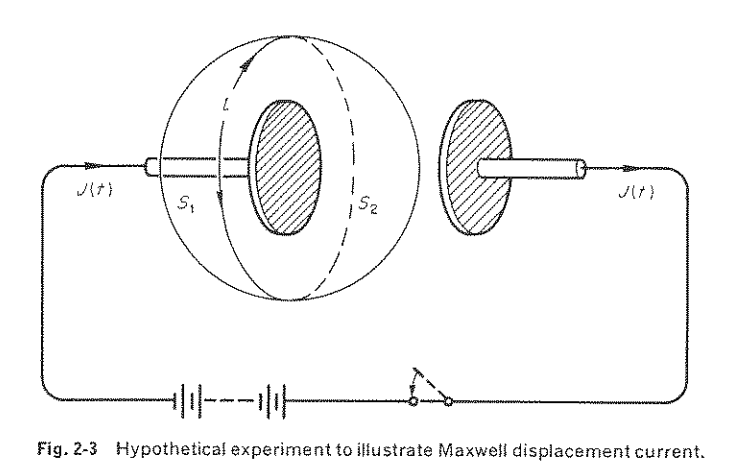
\includegraphics[scale=1]{4.png}
\end{center}
Finally, if we include a component of $\vv{E}$ parallel to $\vv{B}$, we find in the transformed frame, a helix of quadratically increasing pitch:
\newline \begin{equation*}
\begin{aligned}
\vv{v}^1_{||} = \frac{q \, E_{||}}{m} \, t + \vv{v}^1_{o, ||}
\end{aligned}
\end{equation*}\newline
In the laboratory frame, this transforms into a parabolically displaced helix, whose axis lies in the $\vv{B}$, $\vv{E} \times \vv{B}$ plane.
\newpage
We will now shift focus to the \textbf{Magnitude and Direction of an $\bf{E\times B}$ Drift}

The magnitude and direction of the guiding center drift can be
found from Lorentz Equation from Section 2 Equation 66.

To begin, we chose to ignore $m \, \frac{\mathrm{d}\vv{v}}{\mathrm{d}t}$ since it only gives gyromotion and not drift. Also recall from Equation 15 that the drift was independent of time.
\newline \begin{equation*}
\begin{aligned}
\vv{E} + \vv{v} \times \vv{B} = 0 &\quad \Rightarrow \quad & \vv{E} = - \vv{v} \times \vv{B} \\ \\
\vv{E} \times \vv{B} = \vv{B} \times (\vv{v} \times \vv{B}) &\quad =\quad & \vv{v} B^2 - \vv{B} (\vv{v} \cdot \vv{B})
\end{aligned}
\end{equation*}\newline
However, we want the transverse component only. As a result, we get:
\newline \begin{equation}
\begin{aligned}
\vv{v}_{E \times B} = \frac{\vv{E} \times \vv{B}}{B^2} \qquad \text{Where B is the magnitude of the B-field}
\end{aligned}
\end{equation}\newline
The magnitude of which is...
\newline \begin{equation}
\begin{aligned}
|\vv{v}_{E \times B}| = \frac{E}{B}
\end{aligned}
\end{equation}\newline
PHYSICALLY, what gives rise to this motion?
\begin{enumerate}
\item Ion begins to accelerate in an E-field. 
\item This causes $v_{\perp}$ to increase and the instantaneous Larmor radius to also increase.
\item This causes the magnetic force to increase (since force, $\vv{v} \times \vv{B}$,  is perpendicular to the velocity), causing the ion to turn.
\item This causes the Ion to turn so much that its velocity is now opposing $\vv{E}$, thereby going against $\vv{E}$.
\item This now causes the ion to slow down, meaning it decelerates and its instantaneous Larmor radius decreases.
\item The Magnetic force still causes ion to turn, eventually it gets turned
back around such that velocity is aligned with Efield, and the
process repeats.
\end{enumerate}
\newpage
This interaction of the electric and magnetic forces on the charged
particle cause motion that looks like:
\begin{center}
\vspace{70mm}
\textbf{Figure 3}
\end{center}
Finally, note that VExB is independent of q, m, $\vv{v}_{\perp}$
\newpage
\subsection{Arbitrary Force Drift}
The results of the previouse section are actually a special case. They
are the special case for when an Electric force is present with a
Magnetic force. In other words, when an electric field is present
with a magnetic field.

More generally, a charged particle drift occurs when any other force
is present with the magnetic force.

Generic Equation of Motion:
\newline \begin{equation}
\begin{aligned}
m \frac{\mathrm{d}\vv{v}}{\mathrm{d}t} = F + q \, \vv{v} \times \vv{B} 
\end{aligned}
\end{equation}\newline
Where $F$ is any other applied force and $q \, \vv{v} \times \vv{B} $ is the applied magnetic force. From this:
\begin{shaded}
\textbf{Arbitrary Force Drift}
\newline \begin{equation}
\begin{aligned}
\vv{v}_F = \frac{1}{q} \, \frac{\vv{F} \times \vv{B}}{B^2}
\end{aligned}
\end{equation}\newline
\end{shaded}
if $\vv{F} = q \, \vv{E}$ then
\newline \begin{equation*}
\begin{aligned}
\vv{v} = \frac{\vv{E} \times \vv{B}}{B^2} \qquad \qquad \text{Equation 16}
\end{aligned}
\end{equation*}\newline
What if instead we used gravity, $\vv{F}_g = m \, \vv{g}$. Then:
\newline \begin{equation}
\begin{aligned}
\vv{v}_{F_{g}} = \frac{m}{q} \, \frac{\vv{g} \times \vv{B}}{B^2}
\end{aligned}
\end{equation}\newline
\newpage
\subsection{Non-Uniform Fields}
Still more drifts resulting from nonuniform fields can be
superimposed on these motions. For instance:
\begin{shaded}
\textbf{Grad-B drift}
\newline \begin{equation}
\begin{aligned}
\vv{V}_{\nabla B} = \pm \frac{1}{2} \, v_{\perp} \, r_L \frac{\vv{B} \times \nabla B}{B^2}
\end{aligned}
\end{equation}\newline
Which is the case for a non-uniform magnetic field: 
\end{shaded}
In addition we can have:
\begin{shaded}
\textbf{Curvature drift}
\newline \begin{equation*}
\begin{aligned}
\vv{V}_R = \frac{m v_{||}^2}{q \, B^2} \, \frac{\vv{R}_c \times \vv{B}}{R_c^2}
\end{aligned}
\end{equation*}\newline
Where
\newline \begin{equation*}
\begin{aligned}
R_c &= \text{Magnitude of } \vv{R}_c  \\ \\
B &=  \text{Magnitude of } \vv{B} \\ \\
\vv{R}_c &=  \text{Radius of Curvature of the B-field}
\end{aligned}
\end{equation*}\newline
Which is the case for a non-uniform magnetic field in a vacuum where being in a vacuum results in curved field lines.
\end{shaded}
\newpage
\subsection{Conductivity in Collisionless Plasma}
Considering a two-species plasma (electrons and ions) in simple
crossed E and B fields. Both species move in the same direction
with the same drift velocity ($|\vv{v}_{E \times B}| = \frac{E}{B}$).

Particles have different mass and perpendicular velocity, and thus different gyromotion, meaning they have different cyclotron frequencies and Larmor radii. Despite this however, they all move in the ExB direction with same speed.
\begin{center}
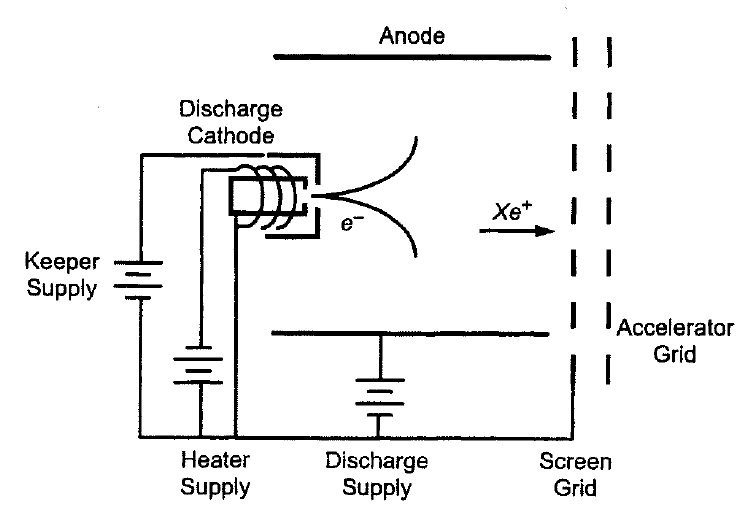
\includegraphics[scale=1.2]{5.png}
\end{center}
Thus, for quasineutrality (\~same number of positive particles as
negative particles), the net current density in the crossed-field
direction is:
\newline \begin{equation*}
\begin{aligned}
\vv{j} = \sum_k n_k \, q_k \, \vv{v}_k = n_i \, q_i \, \vv{v}_i - n_e \, q_e \, \vv{v}_e = 0
\end{aligned}
\end{equation*}\newline
But what if there is a parallel component to the Efield?
\begin{itemize}
\item  $\vv{v}_i \neq \vv{v}_e$; $q \vv{E}$ pulls ions and electrons in opposite
directions.
\item Since we are considering the case with no collisions, we have unopposed acceleration (what is there to stop them? It's
collisionless), which leads to $\vv{v} \rightarrow \infty$ as $t \rightarrow \infty$
\item As a result current becomes ill-defined.
\end{itemize}
Conclusion: Collisions must play an important role in limiting the
unopposed acceleration of the particles.
\newpage
\end{document}